\section{Introduction}
\label{sec:introduction}


\par The objective of this laboratory assignment was to create an audio amplifier circuit. The audio amplifier would recieve an audio input of 10mV (maximum) that would be connected to an 8 Ohm speaker. The source would have an 100 Ohm impedance and the circuit would be supplied with 12 volts by a DC source (Vcc).
\par A good voltage amplifier has to have an high gain $(A_{V})$, a low output impedance $(Z_{o})$ and a high input impedance $(Z_{i})$. So as to meet this criteria the audio amplifier circuit would have two stages: the gain stage and the output stage. This seemed to be the best way to combine the good and not so good properties of each of the amplifier circuits studied in class.\par
 In the gain stage was used a common emitter amplifier with degeneration because it allows us to have a high $Z_{i}$ and a high gain $A_{V}$. Unfortunately the output signal will be degraded because it has a high $Z_{o}$ as well. This problem is to be fixed in the next stage. In this stage an NPN transistor was used.\par
 In the output stage a commom collector amplifier was used in order to maintain the high gain $A_{V}$ from the previous stage whilst having a low $Z_{o}$. This stage is able to maintain the high gain due to the fact that its high input impedance connects to the lower output impedance (but still an high one) of the previous stage and the gain in this section is $\approx 1$. In this stage a PNP transistor was used.
\par   
To determine the quality of the audio amplifier when compared to others, was created a merit classification system. The following equation is the one that gives us the merit of the circuit: 
\begin {equation}
	 MERIT = \frac{Voltage Gain*Bandwidth}{Cost*Lower Cut Off Frequency}   	
	\label{eq:i1}
\end{equation}

and the cost of the components are the following: cost of resistors = 1 monetary unit (MU) per kOhm, cost of capacitors = 1 MU/uF
and cost of transistors = 0.1 MU per diode. 

The general layout of the circuit that was implemented can be seen in \textbf{Figure~\ref{fig:circuit_t4}}
\par
\begin{figure}[h] \centering
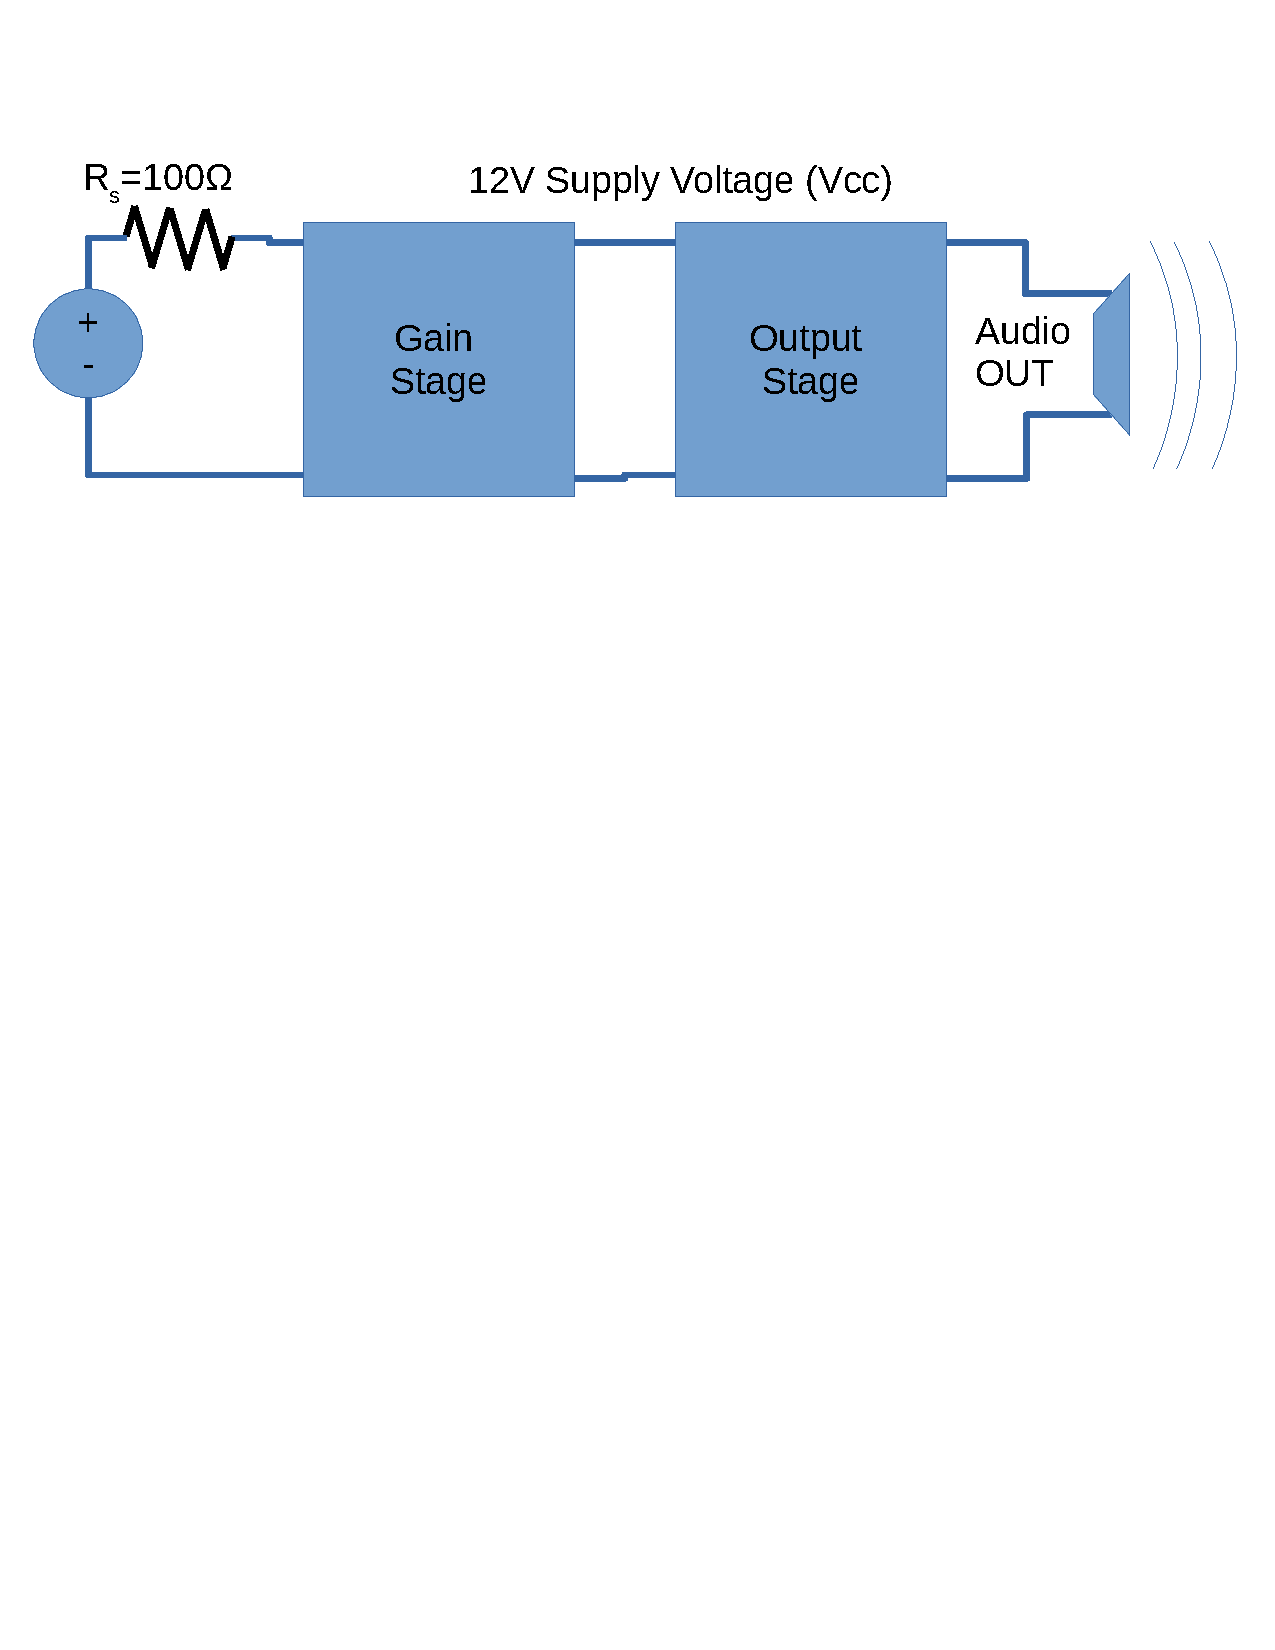
\includegraphics[width=0.6\linewidth]{circuit_t4.pdf}
\vspace{-6cm}
\caption{Circuit in study}
\label{fig:circuit_t4}
\end{figure}


In Section~\ref{sec:analysis}, we present a theoretical analysis of the circuit. Here the circuit is analised using the suitable OP (so as to make sure that the transistors are in the Forward Active Region) and incremental theoretical models studied in the class, in order to predict for each of the stages the gain and the input and output impedances.
In Section~\ref{sec:simulation}, the circuit is analysed by
simulation using the program Ngspice. In Ngspice the Philips BJT'S model BC557A (PNP) and BC547A (NPN) for the transistors were used. The input and output impedances, the lower and upper 3dB cut off frequencies, as well as the gain, were computed by simulation. The conclusions of this study are outlined in
Section~\ref{sec:conclusion}, where the theoretical results obtained in
Section~\ref{sec:analysis} are compared to the simulation results obtained in
Section~\ref{sec:simulation}.





\pagebreak

